\documentclass{article}
\usepackage[a4paper, top=2cm,right=1cm,left=1cm,bottom=0.5cm]{geometry}
\usepackage{url}
\usepackage{amsmath}
\usepackage{ifthen}
\usepackage{xcolor}
\usepackage{amsmath}
\usepackage{tikz} 
\usetikzlibrary{positioning}

\usepackage{xcolor}
\usepackage{listings}
\lstset{
  language=Python,
  breaklines=true,      % allow line breaking
  postbreak=\mbox{\textcolor{red}{$\hookrightarrow$}\space}, % mark wrapped lines
  columns=flexible,      % ← important: keeps syntax highlighting + page breaks
  basicstyle=\ttfamily\footnotesize,
  keywordstyle=\color{blue},
  stringstyle=\color{red},
  commentstyle=\color{gray},
  showstringspaces=false,
  breaklines=true,
  numbers=left,            % ← Line numbers on the left
  numberstyle=\tiny\color{gray}, % Style of line numbers
  numbersep=2pt,        % Space between numbers and code
  inputencoding=utf8,
  extendedchars=true,
  literate={∂}{{\ensuremath{\partial}}}1 {…}{{\ldots}}1
}


\usepackage{multicol}
\usepackage[compact]{titlesec}

\usepackage{mathtools}
\usepackage{siunitx}
\sisetup{inter-unit-product=\ensuremath{{}\cdot{}}, exponent-product = \cdot}
\DeclareSIUnit\bar{bar}

\usepackage[version=4]{mhchem} 

\makeatletter
\newsavebox\myboxA
\newsavebox\myboxB
\newlength\mylenA
\newcommand*\overbar[2][0.75]{%
    \sbox{\myboxA}{$\m@th#2$}%
    \setbox\myboxB\null% Phantom box
    \ht\myboxB=\ht\myboxA%
    \dp\myboxB=\dp\myboxA%
    \wd\myboxB=#1\wd\myboxA% Scale phantom
    \sbox\myboxB{$\m@th\overline{\copy\myboxB}$}%  Overlined phantom
    \setlength\mylenA{\the\wd\myboxA}%   calc width diff
    \addtolength\mylenA{-\the\wd\myboxB}%
    \ifdim\wd\myboxB<\wd\myboxA%
       \rlap{\hskip 0.5\mylenA\usebox\myboxB}{\usebox\myboxA}%
    \else
        \hskip -0.5\mylenA\rlap{\usebox\myboxA}{\hskip 0.5\mylenA\usebox\myboxB}%
    \fi}
\makeatother
\renewcommand{\arraystretch}{1.2}

\makeatletter
\renewcommand*\env@matrix[1][\arraystretch]{%
  \edef\arraystretch{#1}%
  \hskip -\arraycolsep
  \let\@ifnextchar\new@ifnextchar
  \array{*\c@MaxMatrixCols c}}
\makeatother

\usepackage{esint}
\usepackage{setspace}
\usepackage{colortbl}
\usepackage{xcolor}
\usepackage{enumitem}

\usepackage{float}
\usepackage{fancyhdr}
\usepackage{lastpage,refcount, atbegshi}
\usepackage[hidelinks]{hyperref}
\AtBeginShipout{%
  \ifnum\value{page}=\number\numexpr\getpagerefnumber{LastPage}-2\relax
    \phantomsection\label{preLastPage}
  \fi}

% \usepackage{polyglossia}

% \setmainfont{David CLM}
% \setsansfont{Miriam CLM}

% \setdefaultlanguage{english}
% \setotherlanguage{english}  

% \setmathrm{TeX Gyre Schola}

\makeatletter
\def\xpg@set@normalfont#1{%
  \letcs{\rmfamily}{#1@font@rm}%
  \letcs{\sffamily}{#1@font@sf}%
  \letcs{\ttfamily}{#1@font@tt}%
  \def\normalfont{\protect\xpg@select@fontfamily{#1}}%def instead of gdef
  \gdef\reset@font{\protect\normalfont}%
}
% \addto\inlineextras@english{\xpg@set@normalfont{english}}
% \addto\blockextras@english{\xpg@set@normalfont{english}}
\makeatother

\usepackage[style=english]{csquotes}

\usepackage[continuous]{pagenote}
\renewcommand*{\notesname}{NOTE NAME}
\renewcommand{\sectionname}{SECTION NAME}
\renewcommand{\notenuminnotes}[1]{{\textnormal#1. }}
\makepagenote

\renewcommand\text[1]{\textnormal{\textenglish{#1}}}

\setlength{\parindent}{0pt}
\pagestyle{fancy}     % Set the page style to fancy
\fancyhf{}            % Clear all header and footer fields
\renewcommand{\headrulewidth}{0pt} % No line in header
\setlength{\headsep}{0.2cm}% Set the space between header and text

% Define header content
\fancyhead[L]{Page: {\thepage}} % Left header
\fancyhead[R]{\ifthenelse{\value{page}=1}{\today}{} } % Right header shows date on first page

\def\imagewidth{0.9}

\newenvironment{cheatformula}[1][כותרת]{
    \begin{minipage}{\linewidth}
    \textbf{#1}: \\
}{
    % changing vertical  space between every cheat formula
    \end{minipage}\\[0ex]
}

\newcommand{\cheatimage}[4][\imagewidth]{
    \begin{figure}[H]
        \centering
        \includegraphics[width=#1\linewidth]{#2}
        \caption{#3}
        \label{#4}
    \end{figure}
}

\newcommand*{\NameAndID}{%
    \par\noindent\makebox[2in]{\hrulefill} \hspace{0.5in}\makebox[2.0in]{\hrulefill}%
    \par\noindent\makebox[2in][r]{Ramtin Behesht Aeen}      \hspace{0.5in}\makebox[2.0in][r]{ramtinba145822@gmail.com}%
}%

\title{Summary of }
\author{Auther}

\begin{document}

no column mode
% \setlength{\columnsep}{1cm}
% \setlength{\columnseprule}{1pt}

\makeatletter
\begin{center}
    {\NameAndID}\\[2ex]
    {\Large{\textbf{\@title}}}\\[2ex]
\end{center}
\makeatother

% no column mode
% \begin{multicols*}{2}
% \raggedcolumns


\section{Neural Network Theory}
\begin{cheatformula}[Neural Network Structure]

  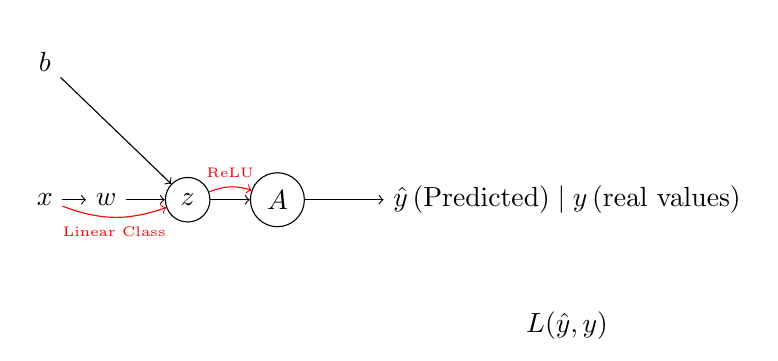
\begin{tikzpicture}[
    node distance=1cm,  % set base distance between nodes
    main/.style = {draw, circle},
    xshift=-2cm
  ]
    \node[main] (z) {$z$};
    \node (x) [left=of z, xshift=-0.3cm] {$x$};          % move x more to the left
    \node (w) [right=of x, xshift=-0.7cm] {$w$};
    \node (b) [above=of x, yshift=3mm] {$b$};            % lift b up a bit from x
    \node[main] (A) [right=of z, xshift=-0.5cm] {$A$};      % A right of z, no extra shift
    \node (y_hat) [right=of A] {$\hat{y} \,\mathrm{(Predicted)} \mid y\, \mathrm{(real\ values)}$};
    \node[below=of y_hat] {$L(\hat{y}, y)$};
    
    \draw[->] (x) -- (w);
    \draw[->] (w) -- (z);
    \draw[->] (b) -- (z);
    \draw[->] (z) -- (A);
    \draw[->] (A) -- (y_hat);

    \draw[->,red] (x) to[bend left=-20] node[midway, below] { \color{red} \tiny Linear Class} (z);
    \draw[->,red] (z) to[bend left=20] node[midway, above] { \color{red} \tiny ReLU} (A);


  \end{tikzpicture}
  
\end{cheatformula}

\begin{cheatformula}[backward pass for w]

  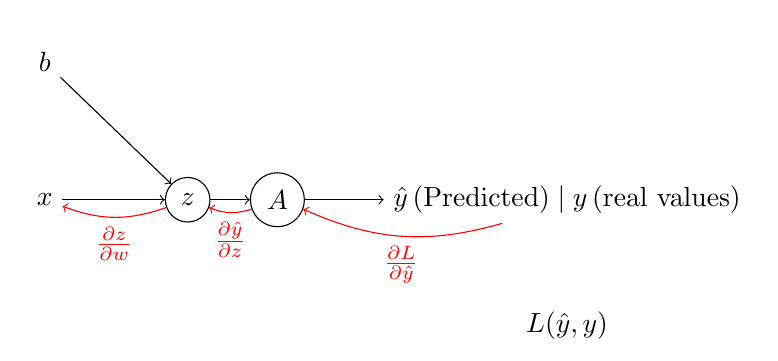
\begin{tikzpicture}[
    node distance=1cm,  % set base distance between nodes
    main/.style = {draw, circle},
    xshift=-2cm
  ]
    \node[main] (z) {$z$};
    \node (x) [left=of z, xshift=-0.3cm] {$x$};          % move x more to the left
    \node (b) [above=of x, yshift=3mm] {$b$};            % lift b up a bit from x
    \node[main] (A) [right=of z, xshift=-0.5cm] {$A$};      % A right of z, no extra shift
    \node (y_hat) [right=of A] {$\hat{y} \,\mathrm{(Predicted)} \mid y\, \mathrm{(real\ values)}$};
    \node[below=of y_hat] {$L(\hat{y}, y)$};
  
    \draw[->] (x) -- (z);
    \draw[->] (b) -- (z);
    \draw[->] (z) -- (A);
    \draw[->] (A) -- (y_hat);
    % Back ward pass:
    \draw[->,red] (y_hat) to[bend left=20] node[midway, below] { \color{red} $\frac{\partial L} {\partial \hat{y}}$} (A);
    \draw[->,red] (A) to[bend left=20] node[midway, below] { \color{red} $\frac{\partial \hat{y}} {\partial z}$} (z);
    \draw[->,red] (z) to[bend left=20] node[midway, below] { \color{red} $\frac{\partial z} {\partial w}$} (x);
  \end{tikzpicture}
  
\end{cheatformula}

\begin{cheatformula}[backward pass for b]

  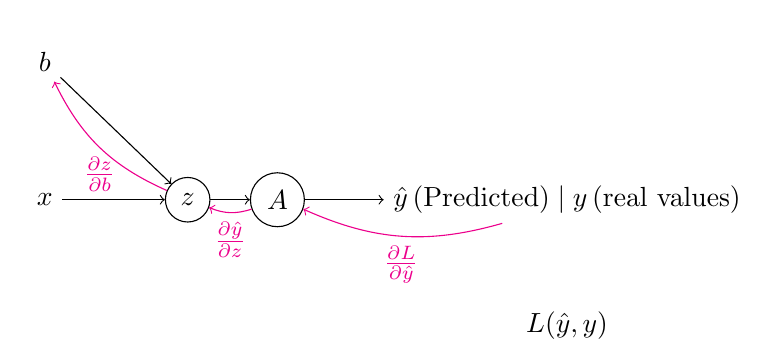
\begin{tikzpicture}[
    node distance=1cm,  % set base distance between nodes
    main/.style = {draw, circle},
    xshift=-2cm
  ]
    \node[main] (z) {$z$};
    \node (x) [left=of z, xshift=-0.3cm] {$x$};          % move x more to the left
    \node (b) [above=of x, yshift=3mm] {$b$};            % lift b up a bit from x
    \node[main] (A) [right=of z, xshift=-0.5cm] {$A$};      % A right of z, no extra shift
    \node (y_hat) [right=of A] {$\hat{y} \,\mathrm{(Predicted)} \mid y\, \mathrm{(real\ values)}$};
    \node[below=of y_hat] {$L(\hat{y}, y)$};
  
    \draw[->] (x) -- (z);
    \draw[->] (b) -- (z);
    \draw[->] (z) -- (A);
    \draw[->] (A) -- (y_hat);
    % Back ward pass:
    \draw[->,magenta] (y_hat) to[bend left=20] node[midway, below] { \color{magenta} $\frac{\partial L} {\partial \hat{y}}$} (A);
    \draw[->,magenta] (A) to[bend left=20] node[midway, below] { \color{magenta} $\frac{\partial \hat{y}} {\partial z}$} (z);
    \draw[->,magenta] (z) to[bend left=20] node[midway, below] { \color{magenta} $\frac{\partial z} {\partial b}$} (b);
  \end{tikzpicture}
  
\end{cheatformula}


\begin{cheatformula}[backward pass for w mathematically]
  \begin{equation}
    L =\underbrace{ L(\underbrace{ \hat{y} \underbrace{ (z(Xw+b)) }_{\frac{\partial z} {\partial w} } }_{\frac{\partial \hat{y}} {\partial z}} )}_{\frac{\partial L} {\partial \hat{y}}}
  \end{equation}
  \begin{equation}
    \frac{\partial L} {\partial w}  = \underbrace{\frac{\partial L} {\partial z}}_{ \frac{\partial L} {\partial \hat{y}}  \frac{\partial \hat{y}} {\partial z} } 
    \frac{\partial z} {\partial w}  
  \end{equation}
  as a Summary:

$$
L = \underbrace{L\left(\hat{y}\right)}_{\frac{\partial L}{\partial \hat{y}}} = \underbrace{L\left(\hat{y}\left(z\right)\right)}_{\frac{\partial L}{\partial \hat{y}} \cdot \frac{\partial \hat{y}}{\partial z}} = \underbrace{L\left(\hat{y}\left(z(XW + b)\right)\right)}_{\frac{\partial L}{\partial \hat{y}} \cdot \frac{\partial \hat{y}}{\partial z} \cdot \frac{\partial z}{\partial W}}
$$

Or more explicitly for the chain rule:

$$
\frac{\partial L}{\partial W} = \frac{\partial L}{\partial \hat{y}} \times \frac{\partial \hat{y}}{\partial z} \times \frac{\partial z}{\partial W}
$$

\begin{itemize}
  \item $z = XW + b$
  \item $\hat{y} = f(z)$ (activation function, e.g. softmax)
  \item $L = loss(\hat{y}, y)$
\end{itemize}

The derivatives $\frac{\partial L}{\partial \hat{y}}$, $\frac{\partial \hat{y}}{\partial z}$, and $\frac{\partial z}{\partial W}$ represent the gradient chain from output all the way down to weights.


  
\end{cheatformula}


\section{Coding the Neural Network}
\begin{cheatformula}[Neural Network Structure]

  \[
  \frac{\partial L}{\partial w} 
  = \frac{\partial L}{\partial \hat{y}} \cdot \frac{\partial \hat{y}}{\partial z} \cdot \frac{\partial z}{\partial w}
  \]
  
  where:
  \begin{itemize}
      \item \textbf{Loss derivative}: $\frac{\partial L}{\partial \hat{y}}$
      \item \textbf{Activation derivative}: $\frac{\partial \hat{y}}{\partial z}$
      \item \textbf{Linear model derivative}: $\frac{\partial z}{\partial w}$
  \end{itemize}
\end{cheatformula}

  \begin{cheatformula}[1. Loss derivative $\left(\frac{\partial L}{\partial \hat{y}}\right)$]
  This is computed in:
  
  \begin{lstlisting}
  def backward(self) -> np.ndarray:  # CrossEntropy
      grad = -self.target / self.prediction / self.target.shape[0]
      return grad
  \end{lstlisting}
  
  \begin{itemize}
      \item \texttt{self.prediction} = $\hat{y}$ (output of softmax)
      \item This gives the gradient from the loss with respect to the softmax output $\hat{y}$.
  \end{itemize}
  \end{cheatformula}
  
  \begin{cheatformula}[Activation derivative $\left(\frac{\partial \hat{y}}{\partial z}\right)$]
  If you have a \texttt{Softmax} layer:
  
  \begin{lstlisting}
  def backward(self, up_grad: np.ndarray) -> np.ndarray:  # Softmax
      ...
      down_grad[i] = np.dot(jacobian, up_grad[i])
  \end{lstlisting}
  
  \begin{itemize}
      \item \texttt{up\_grad} is $\frac{\partial L}{\partial \hat{y}}$ from the loss.
      \item The softmax Jacobian gives $\frac{\partial \hat{y}}{\partial z}$.
      \item Output \texttt{down\_grad} is $\frac{\partial L}{\partial z}$.
      \item This matches step 2 of the chain rule.
  \end{itemize}
  \end{cheatformula}
  
  \begin{cheatformula}[Linear model derivative $\left(\frac{\partial z}{\partial w}\right)$]
  In your \texttt{Linear} layer:
  
  \begin{lstlisting}
  def backward(self, up_grad: np.ndarray) -> np.ndarray:  # Linear
      self.dw = np.dot(self.inp.T, up_grad)  # ∂L/∂w
      self.db = np.sum(up_grad, axis=0, keepdims=True)  # ∂L/∂b
      down_grad = np.dot(up_grad, self.w.T)  # ∂L/∂input
      return down_grad
  \end{lstlisting}
  
  \begin{itemize}
      \item \texttt{up\_grad} is $\frac{\partial L}{\partial z}$ from the activation.
      \item Multiplying with \texttt{inp.T} applies $\frac{\partial z}{\partial w}$ to get $\frac{\partial L}{\partial w}$.
      \item This is step 3 of the professor’s chain rule.
  \end{itemize}

  
  \noindent\textbf{Full Chain in Code:}
  \begin{enumerate}
      \item Loss backward $\rightarrow$ \texttt{CrossEntropy.backward()}
      \[
      \frac{\partial L}{\partial \hat{y}}
      \]
      \item Activation backward $\rightarrow$ \texttt{Softmax.backward()}
      \[
      \frac{\partial L}{\partial z} = \frac{\partial L}{\partial \hat{y}} \cdot \frac{\partial \hat{y}}{\partial z}
      \]
      \item Linear backward $\rightarrow$ \texttt{Linear.backward()}
      \[
      \frac{\partial L}{\partial w} = \frac{\partial L}{\partial z} \cdot \frac{\partial z}{\partial w}
      \]
  \end{enumerate}

  \end{cheatformula}
    
  
  
  


\begin{cheatformula}[Linear]
Abstract Python Code for Layer:
\begin{lstlisting}
  class Layer:
    def __init__(self):
        self.inp = None
        self.out = None

    def __call__(self, inp: np.ndarray) -> np.ndarray:
        return self.forward(inp)

    def forward(self, inp: np.ndarray) -> np.ndarray:
        raise NotImplementedError

    def backward(self, up_grad: np.ndarray) -> np.ndarray:
        raise NotImplementedError

    def step(self, lr: float) -> None:
        pass
\end{lstlisting}

\begin{itemize}
  \item[$\circ$] Input features:
  \begin{equation}
a  
  \end{equation}

  \item[$\circ$] Features weights:
  \begin{equation}
  a
  \end{equation}

  \item[$\circ$] Bias term:
  \begin{equation}
  a
  \end{equation}

  
  \item[$\circ$] Activation function :
  \begin{equation}
  a
  \end{equation}

  
  \item[$\circ$] Output of the neuron:
  \begin{equation}
  y
  \end{equation}
\end{itemize}
\end{cheatformula}


\begin{cheatformula}[explaining Forward in Linear and ReLU]
in Linear and forward class we have:
\begin{lstlisting}
class Linear(Layer):
    ...
    def forward(self, inp: np.ndarray) -> np.ndarray:
        """Perform the linear transformation: output = inp * W + b"""
        self.inp = inp
        self.out = np.dot(inp, self.w) + self.b
        return self.out
  ...
\end{lstlisting}
and in ReLU we have:
\begin{lstlisting}
  class ReLU(Layer):
    def forward(self, inp: np.ndarray) -> np.ndarray:
        """ReLU Activation function: f(x) = max(0, x)"""
        self.inp = inp
        self.out = np.maximum(0, inp)
        return self.out
    
    def backward(self, up_grad: np.ndarray) -> np.ndarray:
        """Backward pass for ReLU: derivative is 1 where input > 0, else 0."""
        down_grad = up_grad * (self.inp > 0)  # Efficient boolean indexing
        return down_grad

\end{lstlisting}
then we make a list of layers like this:
\begin{lstlisting}
layers = [
    Linear(input_size, hidden_size),
    ReLU(),
    Linear(hidden_size, output_size)
]
#passing layers to MLP Class:
model = MLP(layers, CrossEntropy(), learning_rate=0.001) 
\end{lstlisting}
and this list of layers will be called in the MLP class as following:
\begin{lstlisting}
  class MLP:
    def __init__(self, layers: list[Layer], loss_func: Loss, learning_rate: float) -> None:
        self.layers        = layers
        self.loss_func     = loss_func
        self.learning_rate = learning_rate
    
    def __call__(self, input: np.ndarray) -> np.ndarray:
        return self.forward(input)
    
    def forward(self, input: np.ndarray) -> np.ndarray:
        """ pass input through each layer sequentially """
        for layer in self.layers:
            input = layer.forward(input)
        return input
\end{lstlisting}
so the list of layers will be called one by one and the output of each layer will be feed to
the next layer as input. the next simple example will show how it works:
\end{cheatformula}

\begin{cheatformula}[simple example of forward pass]
\begin{lstlisting}
import numpy as np
# Input (batch of 2 samples, each with 3 features)
X = np.array([[1, 2, 3],
              [4, 5, 6]])

# Linear layer
class Linear:
    def __init__(self, in_features, out_features):
        self.W = np.ones((in_features, out_features))  # just ones for simplicity
        self.b = np.zeros((1, out_features))
    
    def forward(self, x):
        z = x @ self.W + self.b
        print("Linear output z =", z)
        return z

# ReLU layer
class ReLU:
    def forward(self, x):
        a = np.maximum(0, x)
        print("ReLU output a =", a)
        return a

# --- Build network ---
layers = [Linear(3, 2), ReLU()]

# --- Forward pass ---
out = X
for layer in layers:
    print(out)
    out = layer.forward(out)
    print("After layer forward, out =", out)

print("Final output =", out)
\end{lstlisting}
First $X$ is set to $\begin{bmatrix}1 & 2 & 3 \\ 4 & 5 & 6\end{bmatrix}$, 
$W$ is set to ones, and $b$ is set to zeros.

\begin{enumerate}
  \item In \texttt{out = layer.forward(out)} the first layer is Linear, and 
  \texttt{out} is equal to $X$. The matrix $X$ will be fed into the Linear 
  \texttt{forward} function.

  \item In the Linear \texttt{forward} function: the output $z$ will be 
  calculated as: 
  \[
    z[0] = [1+2+3, \; 1+2+3] = [6, 6], \quad
    z[1] = [4+5+6, \; 4+5+6] = [15, 15]
  \]

  \item In this step, \texttt{out} will be equal to the output of 
  \texttt{layer.forward(out)}, which is $z$.

  \item Now in the next step of the loop, $z$ will be fed to the ReLU 
  \texttt{forward} function, which is 
  \[
    a = \max(0, x)
  \]
  and it will be equal to 
  \[
    \begin{bmatrix} 6 & 6 \\ 15 & 15 \end{bmatrix}
  \]

  \item Then the result will be printed as: 
  \[
    \texttt{Final output = [[6. 6.] [15. 15.]]}
  \]
\end{enumerate}
\end{cheatformula}

% no column mode
% \end{multicols*}


\newpage

\end{document}